%\section{Introduction}

\section{\centering Introduction - Proxima b et la recherche de vie ailleurs}
%Introduction ou contexte ? j'hésite
\setlength{\columnsep}{1.3em}%
\begin{wrapfigure}[15]{r}{0.45\textwidth}
    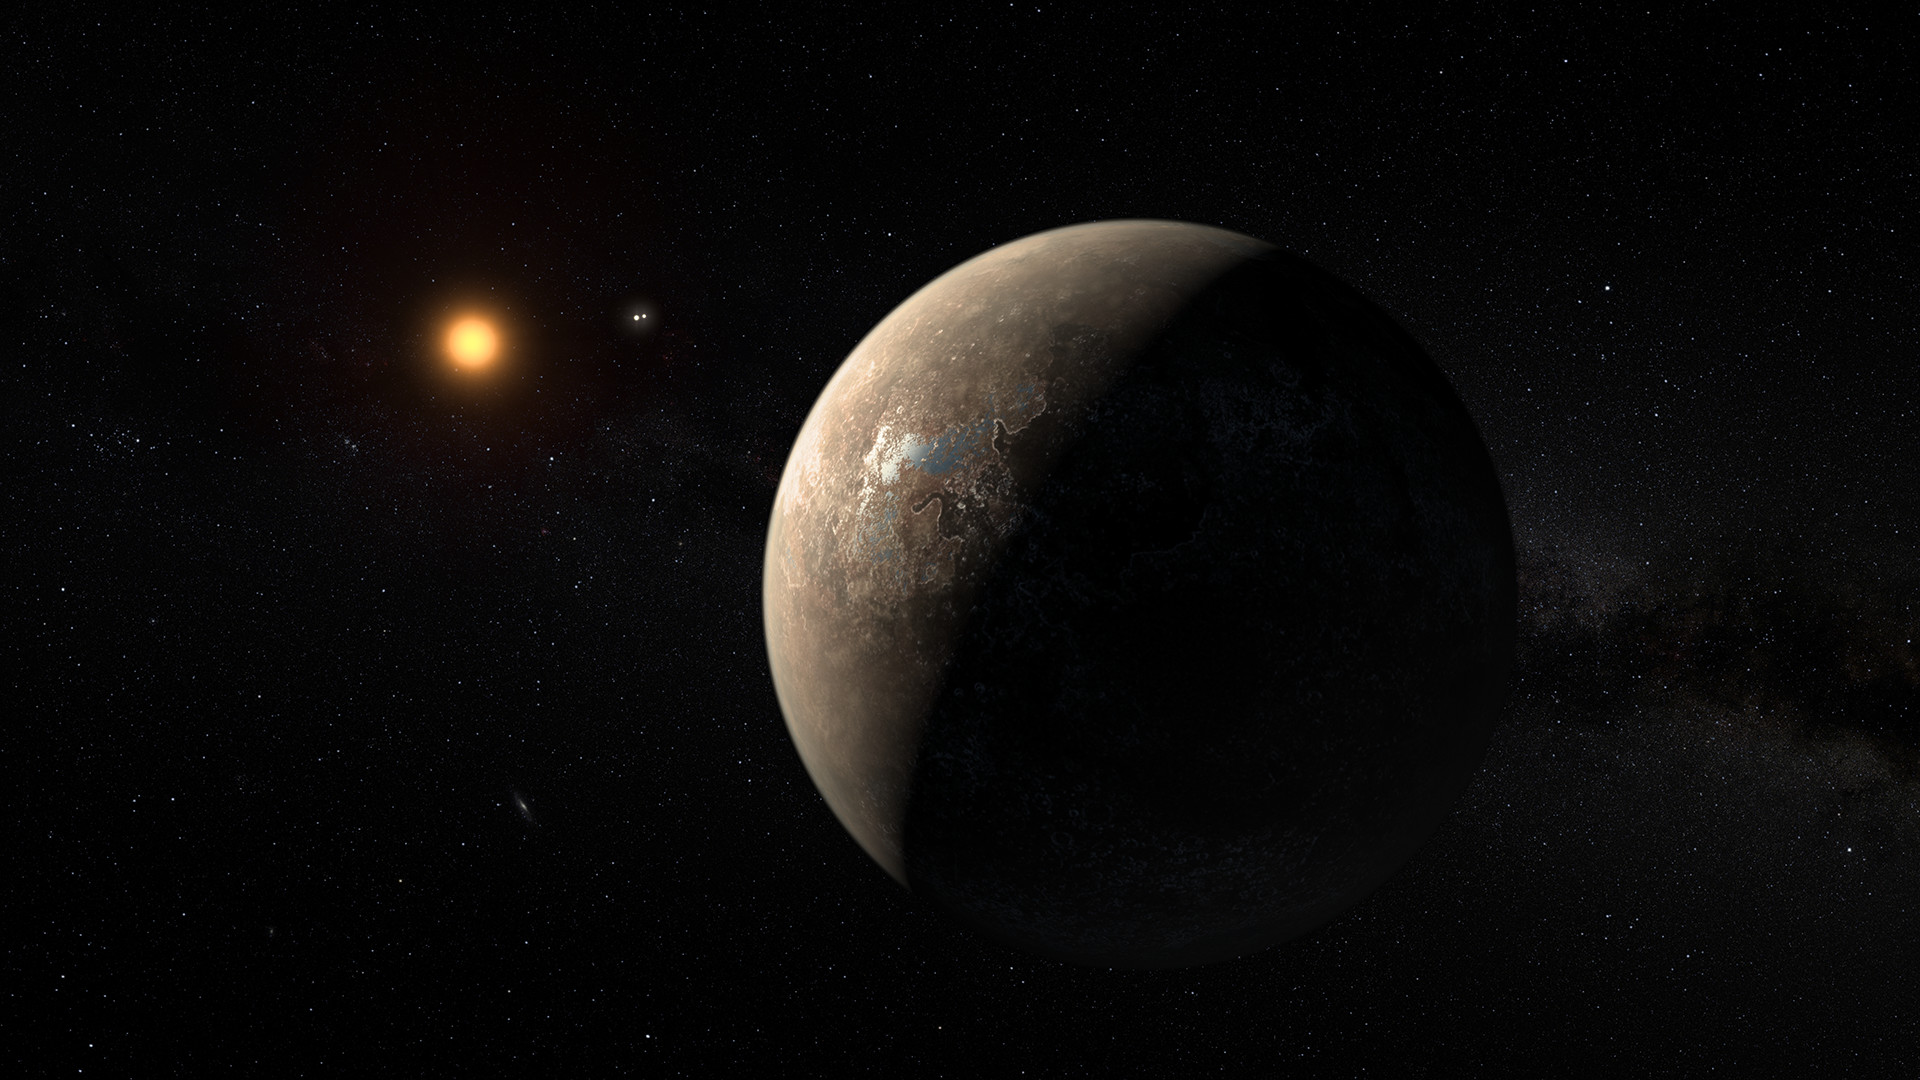
\includegraphics[width=0.45\textwidth]{figures/art_proxb.jpg}
    \caption{Vue d'artiste de Proxima Centauri b, l'exoplanète la plus proche de notre système solaire.}
\end{wrapfigure}

La recherche de planètes habitables a été identifié comme une des priorités majeures dans le secteur de l'astrophysique selon le \textsl{Pathways to Discovery in Astronomy and Astrophyics for the 2020s} [Source]. En effet, la découverte de vie dans notre univers serait une avancée majeure pour l'humanité, et permettrait de répondre à des questions fondamentales sur notre place dans l'univers. 

Parmi les plus de 5000 exoplanètes découvertes à ce jour se trouve \textsl{Proxima b}, une exoplanète de type tellurique découverte en 2016, située dans la zone habitable de son étoile hôte Proxima Centauri. Étant donné sa proximité avec la Terre (à seulement 4.24 années-lumière), Proxima b est une cible de choix pour l'étude de planètes habitables. Non seulement l'étude de cette exoplanète pourrait nous permettre de mieux comprendre les processus de formation et d'évolution des exoplanètes de type terrestres, mais la caractérisation de son atmosphère pourrait également nous permettre l'étude de potentielles biosignatures.

La possibilité de vie aussi proche de nous serait une découverte particulièrement marquante et symbolique pour l'humanité. Cette exoplanète est donc une cible privilégiée pour la recherche de signes de vie. Cependant, l'observation directe de cette exoplanète est rendue difficile par la faible séparation angulaire entre l'étoile et l'exoplanète. Située à une séparation angulaire de 35 mas de son étoile hôte, la situation est similaire à pouvoir distinguer 2 objets à 6 mètres d'écart sur la Lune depuis la Terre. Il est donc nécessaire de développer des techniques d'observation adaptées pour pouvoir caractériser les exoplanètes proches de leurs étoile hôte.

Pour résoudre ce problème, l'ELT-HARMONI, un spectrographe de première lumière observant dans le visible et l'infrarouge (de 0.47 à 2.45 µm) prévu pour le télescope géant européen ELT, est équipé d'un Module Haut Contraste (HCM) développé à l'IPAG. Ce module permettra l'imagerie directe d'exoplanètes jusqu'à $10^{-6}$ fois plus faible que leur étoile hôte, et d'une séparation angulaire de 100 mas. Pour des raisons techniques (lesquels ?), l'observation est limité dans la bande H, soit entre 1.4 et 1.8 µm.


Bien que les masques d'apodisations actuels permettent d'observer des contrastes de l'ordre de $10^{-10}$ pour des planètes assez éloignées et $10^{-5}$ pour des planètes proches, ils sont limités par le flou d'\textsl{optique adaptative}. Ce flou, provoqué par le mouvement des miroirs venant corriger l'impact de l'atmosphère sur la lumière, limite le contraste maximal atteignable par l'ELT-HARMONI.

À l’aide de simulation réalisé dans l’approximation d’un flou d’optique adaptative uniforme dans notre champ de vue (1.), et d’une simulation plus réaliste avec de réels donnée de simulation d’OA (2.), nous calculerons le gain en SNR des images de contrastes générés (PSF) pour une série d’apodiseur adéquat à l’observation de Proxima b.

Pour ces deux situations, nous déterminerons le meilleur apodiseur, défini par le plus grand gain en SNR atteignable. En effet, plus grand est le gain en SNR, plus grand est le gain de temps de télescope, proportionnel au carré du gain en SNR.

%Conclusion 
% On pourra donc gagner un certain temps de téléscope mais on est en définitive limité par un flou d’OA. Si on pouvait réduire le flou jusqu’à $10^(??)$, alors on pourrait espérer pouvoir augmenter le gain de SNR jusqu’à ???


% En effet, ces planète étant généralement très proche de leurs étoiles (car leurs zone habitable sont de l’ordre de $$a=1\text{ UA}$$ comme la Terre en gros), et donc distinguer la lumière de la planète qui est 10^7 fois plus faible que celle de son étoile est un vrai challenge, au vu des distances angulaire à surmonter.

% %Ce qu'on sait déjà
% Une méthode pour surmonter ce problème est l’apodisation : on va venir créer une zone de haut contraste dans la lumière de l’étoile afin de permettre la récupération par l’instrument de la lumière de la planète, permettant de récupérer ces données et analyser la lumière réfléchis de cette planète pour analyser son atmosphere

% Les masques d’apodisations actuelles permettent d’observer jsuqu’a des 10-10 pour des planète assez éloigné et 10-5. Leurs paramètres sont (1.) IWA, (2.) OWA, (3.) T, et (4.) potentiel forme de la dark zone

% %Ce qu'on sait déjà - Limitation par le flou d'OA
% Nous verrons que bien que nous arrivons à atteindre de tes gros contraste, nous sommes limité par l’oa, qui vient créer un flou et limitant le contraste maximale atteignable par l’ELT-HARMONI, instrument sur lequel nous baserons nos recherche et simulation.

% %Méthodes
% À l’aide de simulation (1). réalisé dans l’approximation d’un flou d’optique adaptative uniforme dans notre champ de vue, et (2). d’une simulation plus réaliste avec de réels donnée de simulation d’OA, nous calculerons le gain en SNR des images de contrastes générés (PSF) pour une série d’apodiseur adéquat à l’observation de Proxima b.

% Pour ces deux situations, nous déterminerons le meilleur apodiseur

% Pour résumer, j’ai comparer des rapport de SNR d’apodiseur pour déterminer lequel était le meilleur pour l’observation de Proxima b

% - Il faut qu’il soit le plus grand possible (car $SNR^2$ = temps de téléscope en moins)

% - Il faut qu’il se trouve dans un certain intervalle de longueur d’onde

% - Il faut qu’on puisse récupérer toute l’information lumineuse de la planète pour toutes les longueurs d’onde d’observation

% %Résultats 
% Nous verrons qu’un masque optimal obtenu dans ce cadre de recherche correspond à un apodiseur de paramètres IWA = 2.6 OWA = 6.5 T = 0.70 sans bowtie 

% %Conclusion 
% On pourra donc gagner un certain temps de téléscope mais on est en définitive limité par un flou d’OA. Si on pouvait réduire le flou jusqu’à $10^(??)$, alors on pourrait espérer pouvoir augmenter le gain de SNR jusqu’à ???

% \subsection{Proxima et Proxima b, caractéristiques et intérêts d'observation}
% Résumé de l'article
% \begin{abstract}
% Ceci est le résumé de mon article.
% \end{abstract}

% Introduction
% \section*{Contexte}
% Depuis la découverte de la première exoplanète en 1995, plus de 5000 exoplanètes ont été découvertes. Parmi elles se trouve Proxima Centauri b, une exoplanète de type tellurique située dans la zone habitable de son étoile hôte, Proxima Centauri. Cette exoplanète est donc une cible privilégiée pour la recherche de signes de vie. Cependant, l'observation directe de cette exoplanète est rendue difficile par la faible séparation angulaire entre l'étoile et l'exoplanète. Il est donc nécessaire de développer des techniques d'observation adaptées pour pouvoir caractériser cette exoplanète.\\ 

% ELT-HARMONI est un spectrographe de première lumière observant dans le visible et l'infrarouge (de 0.47 à 2.45 µm) prévu pour le télescope géant européen ELT. Le Module Haut Contraste (HCM), développé à l'IPAG, permettra l'imagerie directe d'exoplanètes jusqu'à $10^{-6}$ fois plus faible que leur étoile hôte, et d'une séparation angulaire de 100 mas %\cite{SystemAnalysis} \cite{ZELDA}.

% \section*{Objectif}
% Pour ceci, on se propose de rechercher un masque de transmission adapté à l'observation de Proxima Centauri b. L'objectif est de trouver un masque de transmission qui permet de réduire le flux de l'étoile tout en conservant le flux de l'exoplanète.

% % Contenu de l'article
% \section{Section 1}
% Contenu de la section 1.

% %\Sfrac{1}{2}

% \section{Section 2}
% Contenu de la section 2.

% % Conclusion
% \section{Conclusion}
% Ceci est la conclusion de mon article.